\section{Sets}

\begin{frame}{Set: collection of objects}
  \begin{itemize}
    \setlength\itemsep{4mm}
    \item Denoted by capital letters: $A,B,X$
    \item Objects in a set are called elements.
    \item Elements are denoted by lower case letters: $a,b,x$
    \item Curly braces around elements: $A = \{a_0,a_1,a_2\}$
  \end{itemize}
  \vspace{3mm}
  \begin{exampleblock}{Examples}
    \begin{novspace}
      \begin{flalign*}
      A &= \{ 1, 2, 3 \} \\
      B &= \{ p \mid p \ \textrm{is a prime number} \}
      \end{flalign*}
    \end{novspace}
  \end{exampleblock}
\end{frame} 


\begin{frame}{No order and no count}
  \begin{alertblock}{A set doesn’t maintain an order of its elements:}
      \begin{flalign*}
        & \{1,2,3\} \  = \  \{1,3,2\} \  = \  \{2,1,3\} \  = \   \{2,3,1\}\\
        & = \  \{3,1,2\} \  = \  \{3,2,1\}
      \end{flalign*}
    \end{alertblock}
    \vspace{3mm}
    \begin{alertblock}{An object is either in the set or not:}
      \begin{flalign*}
        & \{1,2,2,3\} \  = \   \{1,2,3\}
      \end{flalign*}
  \end{alertblock}
\end{frame}

\begin{frame}[fragile]{Question: is $1.0$ an element of $\mathbb{Z}$?}

  To a programmer, the answer is likely no, since $1.0$ is a floating-point number and not an integer.
  Compilers will sometimes give errors if you give $1.0$ where an integer is expected.

  \begin{minted}{python}
IPython 6.1.0 -- An enhanced Interactive Python.
Type '?' for help.
In [1]: i = 1.0
In [2]: a = [1,4,9,16]
In [3]: a[i]
TypeError: list indices must be integers or slices,
not float
In [4]: a[int(i)]
Out[4]: 4
  \end{minted}
\end{frame}

\begin{frame}[fragile]{Question: is $1.0$ an element of $\mathbb{Z}$?}
  Most mathematicians, on the other hand, will likely say $1.0$ is an integer.
  To them, $1$ and $1.0$ are just different representations of the same point on a number line.
  They think of $\mathbb{Z}$ as a subset of the real numbers $\mathbb{R}$.
  Every number on the usual number line is a real number, including $\pi$, $1.5$ and $10$.

  \begin{center}
    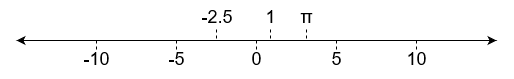
\includegraphics[width=0.8\textwidth]{img/numberline.png} 
  \end{center}

  There's not a lot we can do, other than to provide some context when we consider such sets.
  The discussion can get philosophical, especially in discussions about symbols and semantics.
  Again, this is an important concept in the theory of computation.
\end{frame}



\begin{frame}{Sets containing sets}
  \begin{alertblock}{Subsets}
    \setlength\itemsep{0mm}
    \belowdisplayskip=0pt
    $A$ is a subset of $B$ if all the elements of $A$ are in $B$.
    \begin{flalign*}
      A={1,2,3,4} \qquad   B={2,3} \qquad B \subset A
    \end{flalign*}
  \end{alertblock}

  \begin{alertblock}{Powersets}
    Some sets contain other sets as elements.
    The powerset of a set is the set containing all subsets of it:
    \begin{flalign*}
      A &= {1,2,3} \\
      \mathcal{P}(A) &= \{\{\},\{1\},\{2\},\{3\},\{1,2\},\{1,3\},\{2,3\},\{1,2,3\}\}
    \end{flalign*}
    Note $A$ contains 3 elements and $\mathcal{P}(A)$ contains $2^3=8$.
  \end{alertblock}
\end{frame}


\begin{frame}[fragile]{Famous sets}
  \begin{description}[123]
    \setlength\itemsep{5mm}
    \item[$\mathbb{N}$] -- the natural numbers $\{ 1, 2, 3, \ldots \}$.
    \item[$\mathbb{N}_0$] -- the natural numbers with zero $\{ 0, 1, 2, 3, \ldots \}$.
    \item[$\mathbb{Z}$] -- the integers $\{ \ldots, -2, -1, 0, 1, 2, \ldots \}$.
    \item[$\mathbb{Q}$] -- the rational numbers $\{ \frac{m}{n} \mid m, n \in \mathbb{Z} \}$.
    \item[$\mathbb{R}$] -- the \href{https://en.wikipedia.org/wiki/Real\_number\#Definition}{real numbers}.
    \item[$\mathbb{C}$] -- the complex numbers $\{ a + bi \mid a, b \in \mathbb{R}, i^2 = -1 \}$.
  \end{description}
\end{frame}


\begin{frame}[fragile]{Sizes of sets}
  \begin{topdisp}
  $$ A = \{a,b,c\} \  \Rightarrow \  \vert A \vert = 3 $$
  \end{topdisp}
  \begin{itemize}
    \setlength\itemsep{4mm}
    \item Number of elements is denoted with vertical lines.
    \item The set of all prime numbers is an \emph{infinite} set.
    \item Infinite sets can still have a notion of size.
    \item $\mathbb{R}$ \href{https://en.wikipedia.org/wiki/Cantor\%27s\_diagonal\_argument}{is bigger than} $\mathbb{N}$ even though they're both infinite -- important consequences for computation.
  \end{itemize}
\end{frame}


\begin{frame}{Operations on sets}
  \begin{topdisp}
    $$ A = \{1,2,3\} \qquad  B = \{2,3,4\}$$
  \end{topdisp}
  \vspace{4mm}
  \begin{description}[Intersection:]
    \setlength\itemsep{6mm}
    \item[Union:] $A \cup B = \{1,2,3,4\}$, in $A$ \textbf{or} $B$.
    \item[Intersection:] $A \cap B = \{2,3\}$, in $A$ \textbf{and} $B$.
    \item[Difference:] $A \setminus B = \{1\}$, in $A$ \textbf{not} $B$.
  \end{description}
\end{frame}






\section{Tuples}

\begin{frame}{Tuples: finite list of elements taken from sets}
  \begin{topdisp}
    $$t = (2,1,1) \qquad t \in \mathbb{N} \times \mathbb{N} \times \mathbb{N} \qquad |t| = 3$$
  \end{topdisp}
  \begin{itemize}
    \setlength\itemsep{2mm}
    \item Round brackets denote tuples, and $t$ is a $3$-tuple or a triple.
    \item Tuples have order, and can repeat elements.
    \item Sometimes we omit the brackets and commas: $t = 211$.
    \item $\mathbb{N} \times \mathbb{N} \times \mathbb{N}$ is sometimes shortened to $\mathbb{N}^3$.
    \item The first $\mathbb{N}$ means the first element comes from $\mathbb{N}$.
    \item The second $\mathbb{N}$ means the second element comes from $\mathbb{N}$, etc.
    \item Note that there is a single empty tuple: $()$.
  \end{itemize}
\end{frame}

\begin{frame}[fragile]{Cartesian products of sets}
  \begin{topdisp}
    $$A = \{1,2,3\} \qquad B = \{x,y\}$$
    $$A \times B = \{(1,x),(2,x),(3,x),(2,y),(2,y),(3,y)\}$$
  \end{topdisp}
  
  \begin{itemize}
    \item $A \times B$ is called the cartesian product of $A$ and $B$ -- the set of tuples with first element from $A$ and second from $B$.
    \item $\mathbb{R} \times \mathbb{R} = \mathbb{R}^2$ is the usual 2D plane where we draw plots.
    \item Can extend to any length of tuple: $\mathbb{R}^3$ is the 3D plane.
  \end{itemize}

  \begin{center}
    \resizebox{20mm}{20mm}{%
      \begin{tikzpicture}
        \begin{axis}
          \addplot[color=red]{exp(x)};
        \end{axis}
      \end{tikzpicture}
    }
    \hspace{5mm}
    \resizebox{20mm}{20mm}{%
      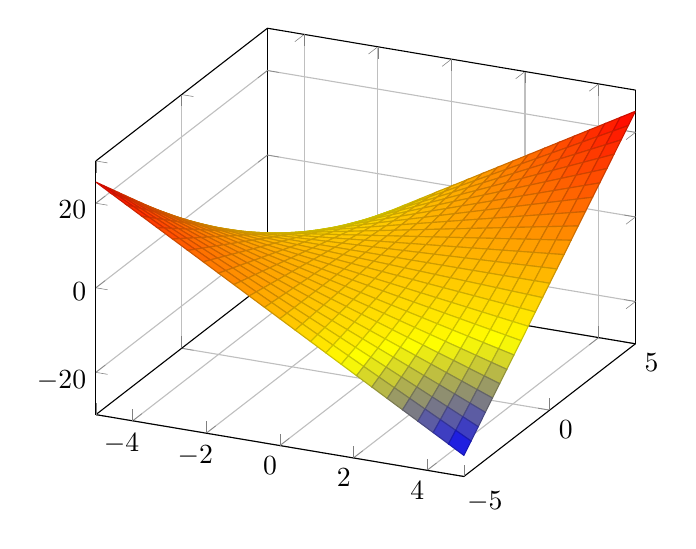
\begin{tikzpicture}
        \begin{axis}[grid=both]
          \addplot3[surf,shader=faceted] {x*y};
        \end{axis}
      \end{tikzpicture}
    }
  \end{center}
\end{frame}

\begin{frame}[fragile]{Multisets}
  \begin{topdisp}
    $$M = \{(a, 2), (b, 10), (x,5) \}$$
  \end{topdisp}
  \begin{itemize}
    \setlength\itemsep{3mm}
    \item We can use sets and tuples to define other data structures.
    \item A multiset over a set $A$ is a subset of $A \times \mathbb{N}$ such that every element of $A$ appears exactly once as the first element in a tuple.
  \end{itemize}
\end{frame}



\section{Maps}

\begin{frame}{Maps}

  \begin{alertblock}{Definition of map}
    A map from a set $A$ to a set $B$ is a subset $M$ of $A \times B$ where each element of $A$ appears as the first element of a tuple in $M$ exactly once.
  \end{alertblock}

  \begin{topdisp}
    $$A = \{a,b,c\} \qquad B = \{x,y,z\}$$
  \end{topdisp}

  \begin{minipage}[t]{0.48\linewidth}
  \begin{exampleblock}{Maps}
    \begin{itemize}
      \item $\{(a,x),(b,x),(c,x)\}$
      \item $\{(a,x),(b,y),(c,z)\}$
    \end{itemize}
  \end{exampleblock}
\end{minipage}
\begin{minipage}[t]{0.48\linewidth}
  \begin{exampleblock}{Not maps}
    \begin{itemize}
      \item $\{(a,x),(a,y),(b,x),(c,x)\}$
      \item $\{(a,x),(b,y)\}$
    \end{itemize}
  \end{exampleblock}
\end{minipage}
\end{frame}


\begin{frame}{One-to-one map}
  \begin{topdisp}
    $$ A = \{1,2,3\} \quad  B = \{a,b,c,d\} \quad  M = \{ (1,a), (2,b), (3,d) \} $$
  \end{topdisp}
  \begin{itemize}
    \setlength\itemsep{3mm}
    \item In a map, $M \subseteq A \times B$, two or more distinct elements of $A$ can be mapped to the same element of $B$.
    \item A map where this does not happen is described as \textbf{one-to-one}.
    \item So, a map in which distinct elements of $A$ go to distinct elements of $B$ is one-to-one.
  \end{itemize}
\end{frame}

\begin{frame}{Onto map}
  \begin{topdisp}
    $$ A = \{1,2,3\} \quad  B = \{a,b,c,d\} \quad  M = \{ (1,a), (2,a), (3,b) \} $$
  \end{topdisp}
  \begin{itemize}
    \setlength\itemsep{3mm}
    \item In a map, not all of the elements of $B$ need to be involved in the map.
    \item A map in which they are all involved is described as \textbf{onto}.
    \item So, a map in which each element of $B$ is paired with an element of $A$ is onto.
  \end{itemize}
\end{frame}

\begin{frame}{Bijections}
  \begin{topdisp}
    $$ A = \{1,2,3\} \quad  B = \{a,b,c\} \quad  M = \{ (1,a), (2,c), (3,b) \} $$
  \end{topdisp}
  \begin{itemize}
    \setlength\itemsep{3mm}
    \item Maps can be neither one-to-one nor onto, one or the other, or both.
    \item A \textbf{bijection} is map that is both one-to-one and onto.
    \item Both $A$ and $B$ must have the same size in a bijection.
  \end{itemize}
\end{frame}


\begin{frame}{Partial maps}
  \begin{topdisp}
    $$ A = \{1,2,3\} \quad  B = \{a,b,c\} \quad  P = \{ (1,a), (3,c) \} $$
  \end{topdisp}
  \begin{itemize}
    \setlength\itemsep{3mm}
    \item A map $M$ from a set $A$ to a set $B$ must involve every element of $A$.
    \item A partial map is like a map, but with that condition relaxed.
    \item A partial map from a set $A$ to a set $B$ is a subset of $A \times B$ where any element of $A$ that appears as the first element in a tuple does so exactly once.
    \item The term \emph{partial map} is a bit of a misnomer, as a partial map is not necessarily a map, but a map is a partial map.
  \end{itemize}
\end{frame}



\section{Languages}


\begin{frame}{Alphabets and strings}
  \begin{itemize}
    \item In some contexts, sets are called alphabets and tuples over them are called strings or words.
    \item We omit the brackets and commas, and the empty tuple is called the empty string and denoted $\epsilon$.
  \end{itemize}

  \begin{exampleblock}{Example}
    Let $A$ be the alphabet $\{0, 1\}$. The following are strings over that alphabet:
      $$ \epsilon, 0, 1, 00, 01, 10, 11, 001, 010, 011, 100, \ldots $$
  \end{exampleblock}

  \begin{exampleblock}{Concatenation}
    We can concatenate strings. For example, concatenating $00$ and $101$ gives $00101$. Technically: $(0,0) \circ (1,0,1) = (0,0,1,0,1)$.
  \end{exampleblock}
\end{frame}


\begin{frame}{Kleene star}
  \begin{topdisp}
    $$ A = \{0,1\} $$
  \end{topdisp}
  
  \begin{description}[abc]
    \item[$A^1$] $= \{0,1\}$, the strings of length one over $A$.
    \item[$A^2$] $= \{00,01,10,11\}$, the strings of length two over $A$.
    \item[$A^i$] $=$ the strings of length $i$ over $A$.
    \item[$A^0$] $= \{\epsilon\}$, the strings of length zero over $A$.
  \end{description}

  \begin{alertblock}{Definition}
    The Kleene star (denoted $A^*$) of $A$ is the union of all the $A^i$:
    $$\bigcup_i A^i = \{ \epsilon, 0, 1, 00, 01, 10, \ldots\}$$
  \end{alertblock}

  \emph{Note the alphabet can be different.}
\end{frame}


\begin{frame}{Languages}
  \begin{topdisp}
    $$ L \subseteq A^* $$
  \end{topdisp}

  Any subset of the star of an alphabet is a \textbf{language}.

  \begin{alertblock}{Operations}

    Create three new languages from two languages $L_1$ and $L_2$.

    \begin{description}[Concatenate:]
      \item[Union:] $L_1 \cup L_2$, all strings in $L_1$ or $L_2$.
      \item[Concatenate:] $L_1 \circ L_2$, join each string in $L_1$ with each in $L_2$.
      \item[Star:] $L_1^*$, the Kleene star of $L_1$ using concatenation.
    \end{description}
  \end{alertblock}

  \emph{We could consider two languages over different alphabets, if we took the union of the alphabets.}
\end{frame}


\begin{frame}{File types as languages}
  \begin{itemize}
    \setlength\itemsep{3mm}
    \item The set of all valid PDF files, according to the PDF specification, is a language over the alphabet $A =\{0,1\}$.
    \item So, the set of valid PDFs is a subset of $A^*$.
    \item So is the set of valid DOCX file.
    \item A computer program that converts PDF files to DOCX files just maps one subset of $A^*$ to another subset of $A^*$.
    \item Remember too, that executable files themselves are stored as files in 0's and 1's.
  \end{itemize}
\end{frame}